\documentclass{article}
\usepackage[a4paper, total={6in, 8in}]{geometry}
\usepackage{listings}
\usepackage{xcolor}
\usepackage{graphicx}
\usepackage{verbatim}
\usepackage{hyperref}
\usepackage{url}
\usepackage[utf8]{inputenc}
\usepackage{float}

\lstset{
  basicstyle=\ttfamily\footnotesize,
  keywordstyle=\color{blue}\bfseries,
  commentstyle=\color{green!50!black},
  stringstyle=\color{red},
  numbers=left,
  numberstyle=\tiny\color{gray},
  stepnumber=1,
  numbersep=5pt,
  tabsize=2,
  breaklines=true,
  breakatwhitespace=false,
  showspaces=false,
  showstringspaces=false,
  showtabs=false,
  frame=single,
  rulecolor=\color{black},
  captionpos=b,
  language=C++,
  morekeywords={},
}

\begin{document}

\title{\textbf{Modern Tetris Implementation:\\Object-Oriented Design \& Documentation}}
\author{By CS23B1023 Athidathan K}
\date{November 11, 2024}
\maketitle
\tableofcontents

\section{Overview}

This documentation provides an overview of the Tetris project, explaining its structure, specifications, and how various Object-Oriented Programming (OOP) concepts are incorporated, including encapsulation, abstraction, inheritance, polymorphism, operator overloading, and plans for future use of templates and virtual functions.

The Tetris project is implemented in C++ using the Raylib graphics library. The game simulates the classic Tetris gameplay, where different shaped blocks fall into a grid, and the player manipulates them to form complete rows.

\section{Project Structure}

\begin{verbatim}
.vscode/
build/
Font/
    Handjet.ttf
lib/
    raylib.h
src/
    block.cpp
    block.h
    blocks.cpp
    colors.cpp
    colors.h
    game.cpp
    game.h
    grid.cpp
    grid.h
    main.cpp
    position.cpp
    position.h
Makefile
Documentation.tex
main.code-workspace
\end{verbatim}

\section{Classes and Files}

\subsection{\texttt{Position} Class (\texttt{src/position.h}, \texttt{src/position.cpp})}

Represents the position of a block in the grid.

\begin{lstlisting}[language=C++]
class Position {
public:
    int row;
    int column;
    Position(int row, int column);
    Position operator+(const Position& other) const ;
};
\end{lstlisting}

\subsection{\texttt{Block} Class Hierarchy (\texttt{src/block.h}, \texttt{src/block.cpp,\texttt{src/blocks.cpp}})}
\subsubsection{Base \texttt{Block} Class}
\textbf{Encapsulation}: The \texttt{Block} class encapsulates the properties and behaviors of a Tetris block.

\begin{lstlisting}[language=C++]
class Block {
public:
    Block();
    void Draw(int offsetX, int offsetY);
    void Move(int rows, int columns);
    void Rotate();
    void UndoRotation();
    std::vector<Position> GetCellPositions();
protected:
    int id;
    int rotationState;
    int rowOffset;
    int columnOffset;
    std::map<int, std::vector<Position>> cells;
    int cellSize;
    std::vector<Color> colors;
};
\end{lstlisting}

\textbf{Example}: The \texttt{Block} class manages its state internally and provides public methods for interaction, demonstrating encapsulation.

\subsection{Derived Block Classes (\texttt{src/blocks.cpp})}

\textbf{Inheritance}: Multiple classes (\texttt{LBlock}, \texttt{JBlock}, \texttt{IBlock}, \texttt{OBlock}, \texttt{SBlock}, \texttt{TBlock}, \texttt{ZBlock}) inherit from the \texttt{Block} class.

\textbf{Example}:

\begin{lstlisting}[language=C++]
// src/blocks.cpp

#include "block.h"

// LBlock class inheriting from Block
class LBlock : public Block {
public:
    LBlock() {
        id = 1;
        cells[0] = {Position(0, 2), Position(1, 0), Position(1, 1), Position(1, 2)};
        cells[1] = {Position(0, 1), Position(1, 1), Position(2, 1), Position(2, 2)};
        cells[2] = {Position(1, 0), Position(1, 1), Position(1, 2), Position(2, 0)};
        cells[3] = {Position(0, 0), Position(0, 1), Position(1, 1), Position(2, 1)};
        Move(0, 3);
    }
};

// Other block classes (JBlock, IBlock, OBlock, SBlock, TBlock, ZBlock) defined similarly
\end{lstlisting}

Each derived class initializes its specific shape by setting up the \texttt{cells} member variable inherited from the \texttt{Block} class.

\subsection{\texttt{Grid} Class (\texttt{src/grid.h}, \texttt{src/grid.cpp})}

Represents the game grid where the blocks are placed. Manages the grid state, drawing, and clearing full rows.

\begin{lstlisting}[language=C++]
// src/grid.h

#pragma once
#include <vector>
#include <raylib.h>

class Grid{
public:
    Grid();
    void Initialize();
    void Print();
    void Draw();
    bool IsCellOutside(int row, int column);
    bool IsCellEmpty(int row, int column);
    int ClearFullRows();
private:
    int grid[20][10];
    int numRows;
    int numCols;
    int cellSize;
    std::vector<Color> colors;
    bool IsRowFull(int row);
    void ClearRow(int row);
    void MoveRowDown(int row, int numRows);
    
friend class Game;
};
\end{lstlisting}

\subsection{\texttt{Game} Class (\texttt{src/game.h}, \texttt{src/game.cpp})}

Controls the overall game logic.

\textbf{Abstraction}: Provides simplified methods to handle game mechanics like input handling and block movement.

\begin{lstlisting}[language=C++]
// src/game.h

#pragma once
#include "grid.h"
#include "block.h"
#include "raylib.h"

class Game {
public:
    Game();
    ~Game();
    void Draw();
    void HandleInput();
    void MoveBlockDown();
    bool gameOver;
    int score;
private:
    void MoveBlockLeft();
    void MoveBlockRight();
    void RotateBlock();
    void LockBlock();
    bool IsBlockOutside();
    bool BlockFits();
    void Reset();
    void UpdateScore(int linesCleared, int moveDownPoints);
    Grid grid;
    Block currentBlock;
    Block nextBlock;
    std::vector<Block> blocks;
};
\end{lstlisting}


\section{OOP Concepts Incorporated}

\subsection{Encapsulation}

Classes manage their own data and expose functionality through public methods. Access specifiers \texttt{public} and \texttt{private} are used to enforce access control, separating the interface from the implementation.

\textbf{Example}:

In the \texttt{Block} class (\texttt{src/block.h}), data members are declared as \texttt{protected} or \texttt{private}, while member functions that form the interface are declared as \texttt{public}.

\begin{lstlisting}[language=C++]
// src/block.h

class Block {
public:
    Block();
    void Draw(int offsetX, int offsetY);
    void Move(int rows, int columns);
    void Rotate();
    void UndoRotation();
    std::vector<Position> GetCellPositions();
protected:
    int id;
    int rotationState;
    int rowOffset;
    int columnOffset;
    std::map<int, std::vector<Position>> cells;
    int cellSize;
    std::vector<Color> colors;
};
\end{lstlisting}

The implementation of these member functions is separated in the corresponding \texttt{.cpp} file (\texttt{src/block.cpp}), keeping the interface clean and promoting encapsulation.

\subsection{Abstraction}

Abstraction is achieved by using header files to define class interfaces. The implementation details are hidden in the \texttt{.cpp} files, allowing users of the classes to interact with them without needing to understand the internal workings.

\textbf{Example}:

The \texttt{Game} class interface is defined in \texttt{src/game.h}, abstracting the game mechanics and providing a clear interface for interaction.

\begin{lstlisting}[language=C++]
// src/game.h

class Game {
public:
    Game();
    ~Game();
    void Draw();
    void HandleInput();
    void MoveBlockDown();
    bool gameOver;
    int score;
private:
    // Private member functions and variables
};
\end{lstlisting}

\subsection{Inheritance}

Inheritance is used to create specialized block types from a base \texttt{Block} class. This allows for code reuse and establishes a hierarchical class structure.

\textbf{Class Hierarchy}:

\begin{itemize}
    \item \texttt{Block} (base class)
    \begin{itemize}
        \item \texttt{IBlock}
        \item \texttt{JBlock}
        \item \texttt{LBlock}
        \item \texttt{OBlock}
        \item \texttt{SBlock}
        \item \texttt{TBlock}
        \item \texttt{ZBlock}
    \end{itemize}
\end{itemize}

\textbf{Example}:

\begin{lstlisting}[language=C++]
// src/blocks.cpp

class TBlock : public Block {
public:
    TBlock() {
        id = 6;
        cells[0] = {Position(0, 1), Position(1, 0), Position(1, 1), Position(1, 2)};
        // other rotation states...
        Move(0, 3);
    }
};
\end{lstlisting}

\subsection{Polymorphism}

Polymorphism allows objects to be treated as instances of their base class rather than their actual derived class. This project demonstrates both compile-time and run-time polymorphism.

\subsubsection{Compile-Time Polymorphism}

\textbf{Function Overloading (used)}:

Function overloading is utilized in the project to allow functions with the same name to have different parameter lists.

\begin{lstlisting}[language=C++]
// src/block.h
class Block {
public:
    void Move(int rows, int columns);
    
    // Overloaded Move function
    void Move(const Position& pos);
};
\end{lstlisting}

\textbf{Operator Overloading (used)}:

Operator overloading is implemented in the \texttt{Position} class to simplify position arithmetic.

\begin{lstlisting}[language=C++]
// src/position.cpp

Position Position::operator+(const Position &other) const{
    return Position(row + other.row, column + other.column);
}
\end{lstlisting}

This allows positions to be added using the \texttt{+} operator.

\textbf{Templates (not currently used)}:

Templates are not explicitly used in this project as the data types are consistent, and there's no immediate need for generic programming. However, templates could be implemented for generic data structures or algorithms if needed in future enhancements.

\subsubsection{Run-Time Polymorphism}

\textbf{Virtual Functions (planned for future use)}:

Virtual functions are intended to be used in future extensions, such as when adding a \texttt{Player} class to extend multiplayer functionality.

\textbf{Example}:

In future development, a \texttt{Player} class could be defined with virtual methods that are overridden by derived classes for different player types (e.g., human player, AI player).

\section{Example Code Snippets}

\subsection{Drawing a Block}

\begin{lstlisting}[language=C++]
// src/block.cpp

void Block::Draw(int offsetX, int offsetY) {
    std::vector<Position> tiles = GetCellPositions();
    for (const Position& item : tiles) {
        DrawRectangle(
            item.column * cellSize + offsetX,
            item.row * cellSize + offsetY,
            cellSize - 1, cellSize - 1,
            colors[id]
        );
    }
}
\end{lstlisting}

Demonstrates encapsulation by handling drawing internally.

\subsection{Handling Block Rotation}

\begin{lstlisting}[language=C++]
// src/block.cpp

void Block::Rotate() {
    rotationState = (rotationState + 1) % cells.size();
}
\end{lstlisting}

Shows how the block manages its rotation state.

\subsection{Moving Blocks Down Automatically}

\begin{lstlisting}[language=C++]
// src/main.cpp

if (EventTriggered(0.2)) { // Game speed is 0.2 seconds
    game.MoveBlockDown();
}
\end{lstlisting}

Demonstrates how the game logic moves the current block down at regular intervals.

\section{Screenshots}
Below are some screenshots demonstrating the gameplay of the Tetris project.

\begin{figure}[H]
    \centering
    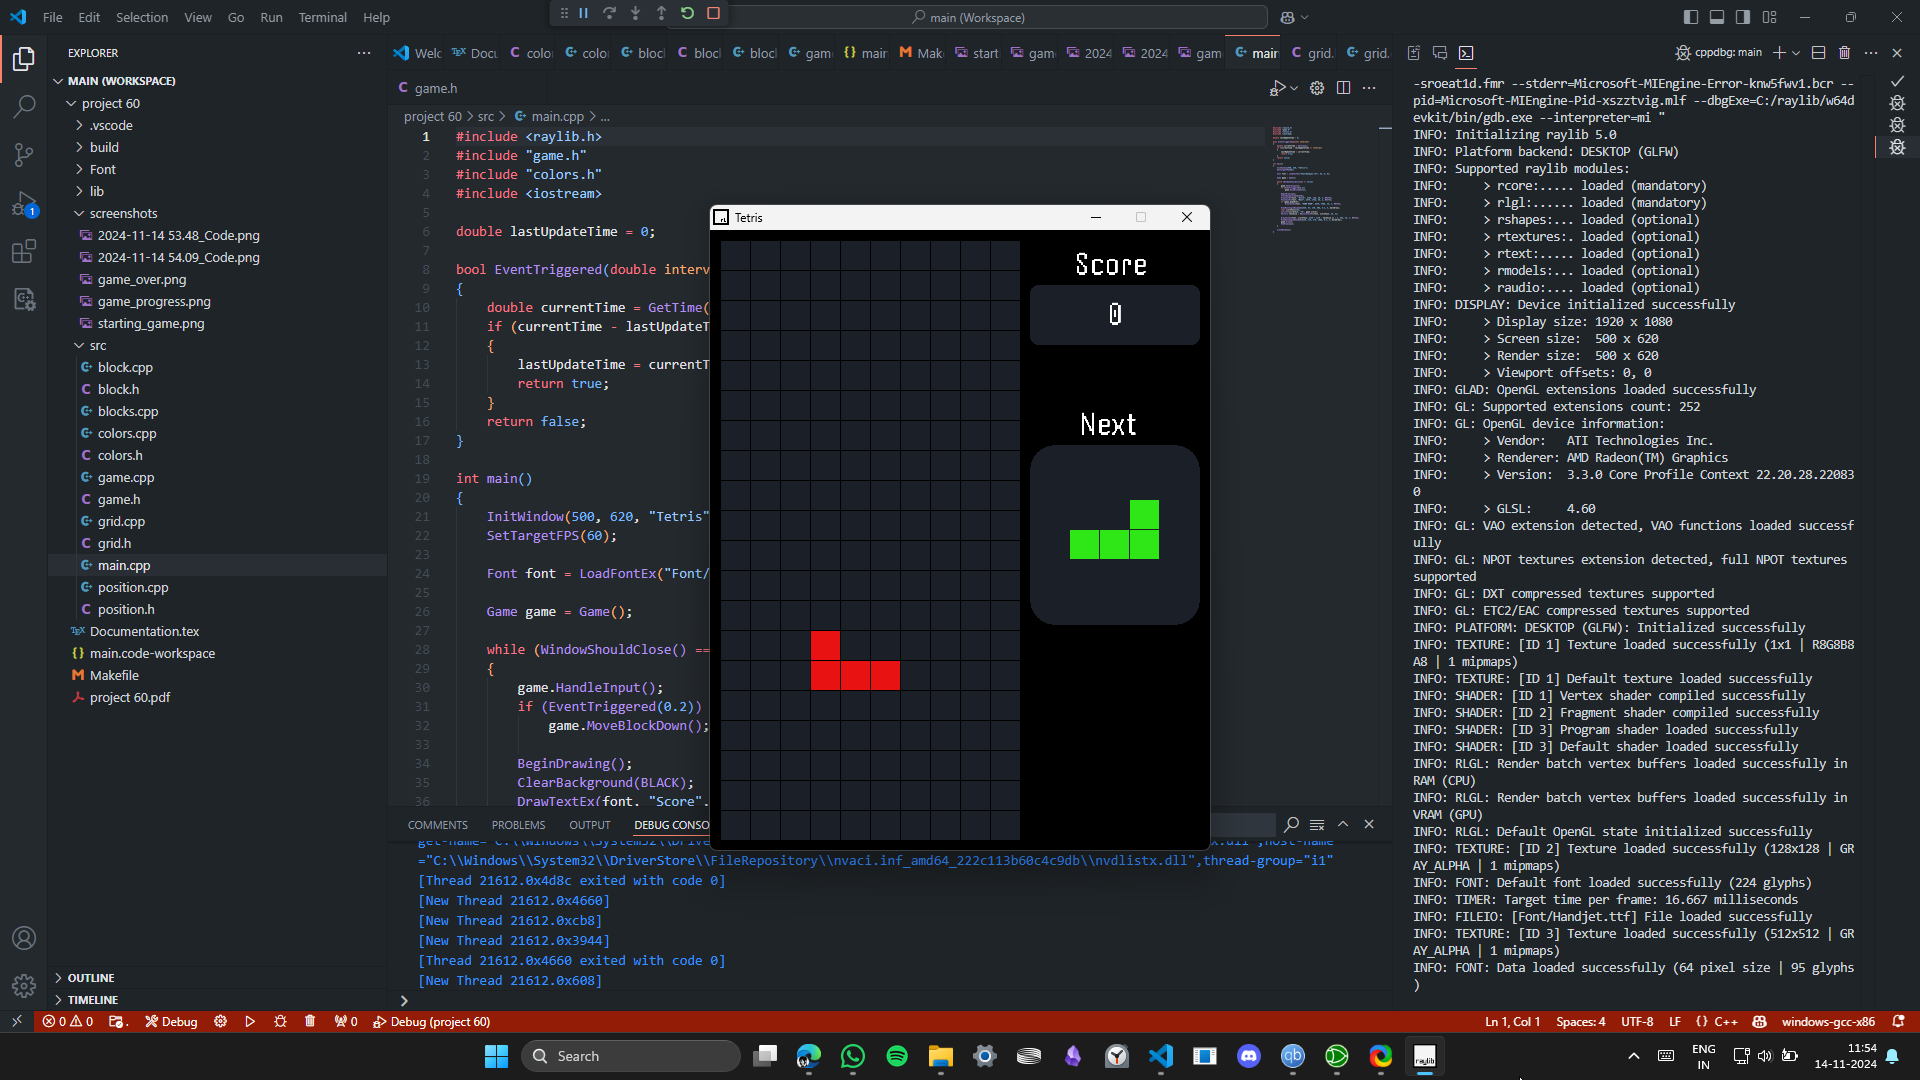
\includegraphics[width=0.8\textwidth]{start.png}
    \caption{Starting the Tetris game}
    \label{fig:screenshot_start}
\end{figure}

\begin{figure}[H]
    \centering
    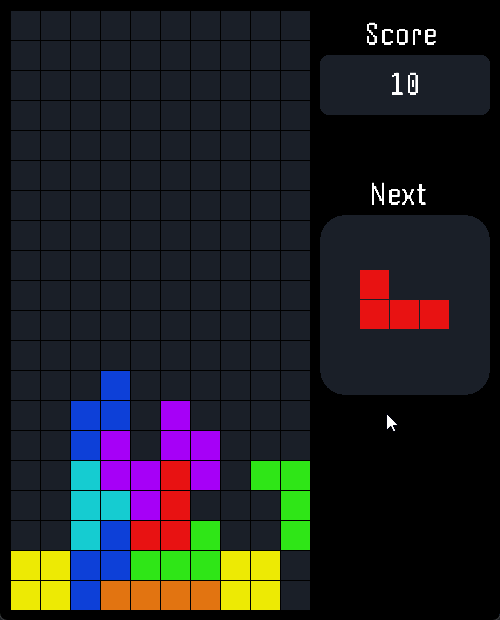
\includegraphics[width=0.8\textwidth]{game_progress.png}
    \caption{Gameplay in progress}
    \label{fig:screenshot_gameplay}
\end{figure}

\begin{figure}[H]
    \centering
    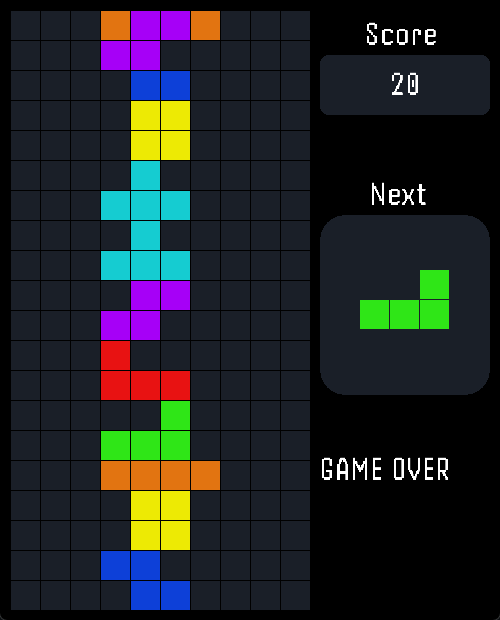
\includegraphics[width=0.8\textwidth]{game_over.png}
    \caption{Game Over screen}
    \label{fig:screenshot_gameover}
\end{figure}
\section{Building the Project}

The project is developed in C++ using the Raylib graphics library, and the instructions are tailored for Windows users.
this project was developed on Windows 10 using MinGW-w64 as the compiler. The instructions assume a similar setup, but the project can be adapted for other platforms with minor modifications. The project can also be downloaded from my github \url{https://github.com/Athidathan/OOPtetris/}

\subsection{Requirements}

\begin{itemize}
    \item \textbf{Operating System}: Windows 10 or higher
    \item \textbf{Compiler}: MinGW-w64 (GCC for Windows) or Microsoft Visual Studio
    \item \textbf{Library}: \href{https://www.raylib.com/}{Raylib} (version 4.0 or higher)
     \item \textbf{Make Build system}: MinGW-w64 includes \texttt{mingw32-make} for building the project using the provided \texttt{Makefile}.
\end{itemize}

\subsection{Instructions}

\begin{enumerate}
    \item Install the required compiler and Raylib library.
    \item Open the Command Prompt and navigate to the project directory:
    \begin{lstlisting}
    cd path\to\your\project
    \end{lstlisting}
    \item Compile the project using the provided \texttt{Makefile}:
    \begin{lstlisting}
    mingw32-make
    \end{lstlisting}
    \item Run the game executable:
    \begin{lstlisting}
    game.exe
    \end{lstlisting}
\end{enumerate}

\begin{verbatim}
make
\end{verbatim}

This command will compile the source files and link the necessary libraries to produce the final executable.

\section{Future Plans}

Looking ahead, there are several enhancements planned to expand the functionality and educational value of this Tetris project:

\begin{itemize}
    \item \textbf{Local Multiplayer}: Implementing a local multiplayer mode where two players can play simultaneously on the same machine. This feature will introduce new dynamics and while incorporating polymorphism.
    \item \textbf{Additional Game Modes}:
    \begin{itemize}
        \item \textbf{Versus Mode}: Players compete against each other, with mechanics such as sending garbage lines to the opponent when clearing multiple lines.
        \item \textbf{Challenge Mode}: Players face progressively increasing difficulty levels with unique challenges.
        \item \textbf{Time Attack Mode}: Players aim to score as high as possible within a limited time frame.
    \end{itemize}
\end{itemize}

\section{Conclusion}

This Tetris project serves as a practical example of implementing OOP concepts in C++. Through encapsulation, abstraction, inheritance, polymorphism, and operator overloading, the project provides a comprehensive introduction to OOP in a game development context.

The project demonstrates how to structure a C++ application using classes and inheritance, how to manage game state and logic, and how to integrate a graphics library (Raylib) to handle rendering and input.

With future enhancements, especially when the game is extended to support multiplayer functionality. The project offers ample opportunities to delve into advanced topics such as networking, artificial intelligence, and improved user interfaces, further enriching the learning experience.
\newpage
\begin{thebibliography}{9}

\bibitem{raylib}
Raylib Official Website. \url{https://www.raylib.com/}

\bibitem{raylib_tutorials}
Raylib Learning Resources. \url{https://github.com/raysan5/raylib/wiki}

\bibitem{tetris}
Tetris Game. \url{https://en.wikipedia.org/wiki/Tetris}
\end{thebibliography}
\end{document}